\section{Description}  
The purpose of the recordings are to obtain several different audio files of music to use for both unit tests and tests on the final system. \\
It is important to know the exact signal on each audio files in order to use it as reference when validating the system. Hence, recording of the audio will take place in the anechoic room provided by the acoustic laboratory at AAU. \\
Musical signals and noise are recorded separately. Hereby specific noise can be added to the music digitally in order to gain further control of the signals. \\
Table \ref{tab:audio} makes a list representing the contents of each audio file to be recorded. The contents of the musical audio files is selected based on the complexity of the frequencies from a single tone to a melody played with chords. \\
Each type of file will be recorded at least two times. This is done to verify the tone played and minimize the human mistakes.    \\
The noise to be recorded is chosen to represent additive noise that could appear naturally in a situation where the final system would be used. Note that convolution noise is disregarded as a result of recording in the anechoic room.

\begin{table}[H]
\centering
\begin{tabular}{l|l|l}
\hline
  & \textbf{Music}                      & \textbf{Noise}     \\ \hline
1 & $E_2$ string of $82.41$ Hz			& Random speak       \\ \hline
2 & $E_2$ string of $329.63$ Hz			& Curling paper      \\ \hline
3 & $E_2$ chord                         & Random clapping    \\ \hline
4 & $E_4$ chord                 		& Rhythmical clapping \\ \hline
5 & Melody of single strings - slow/fast & Random cheering    \\ \hline
6 & Melody with chords - slow/fast      & Singing            \\ \hline
\end{tabular}
\caption{List of recordings in the anechoic room.}
\label{tab:audio}
\end{table}

Beside the listed audio files, which add up to $14$ different types of files, natural outdoor sound is also recorded outside the anechoic room.

\subsection{Anechoic room} 
An anechoic room is designed to absorb all reflections from sound or electromagnetic waves. Further the room is isolated from exterior noise, which makes it possible to only record or measure the exact sound that is made by the musical instrument without the presence of interfering reflections. \\ The specific room at AAU is build as a box inside a box. The inner box is placed on rubber suspensions, and the inner walls are covered by sound absorbing wedges of about 0.4 m in length due to requirements for anechoic performances. The inside dimensions of the room are 4.5 m times 5.0 m with a height of 4.0 m \cite{anechoic}.\\
Hence, by recording in the anechoic room signal noise is reduced to a minimum.

\section{Procedure}
\textbf{Set up inside anechoic room:}\\
\begin{itemize}
\item[-] A grid to support a microphone stand is installed as the only floor in the anechoic room, partly covered by wadding. 
\item[-] One man with a guitar sits on the grid, playing into the microphone. 
\item[-] The microphone is connected through the wall into the control room next to the anechoic room. 
\end{itemize}   
\textbf{Set up in control room: }
\begin{itemize}
\item[-] The microphone is connected to the ADC, which is connected to the PC.
\item[-] The PC is running the recording program Audacity. From the program the sampling frequency is specified to 44.1 kHz.     
\end{itemize}

Table \ref{tab:equip} specifies the equipment used for the recording. Figures \ref{fig:setup1} and \ref{fig:setup2} show the set up inside the anechoic room.
\begin{table}[H]
\centering
\begin{tabular}{l|l|l}
\hline
  & \textbf{Equipment}                & \textbf{Specifications}                                                                                      \\ \hline
1 & Condenser Microphone, C 414 B-ULS &                                                                                                             \begin{tabular}[c]{@{}l@{}}
Frequency Range: $20-20000$ Hz \\ 
Equivalent Noise Level 14 dB-A\\
Electric Impedance: $180$ ohm \end{tabular} \\ \hline
2 & ADC, Roland Quad-capture          & \begin{tabular}[c]{@{}l@{}}Analog $2 \times 2$, digital $2 \times 2$, USB 2.0,\\ 4 in/4 out, 24 bit, 192 kHz\end{tabular} \\ \hline
3 & PC                                &                                                                                                             Lenovo E31-70, Windows 10 \\ \hline
4 & Audacity                          &                                                                                                              \\ \hline
5 & Guitar   	                      &                                                                                                              Takamine ef261san semi acoustic guitar \\ \hline
6 & Paper   	                      &                                                                                                              \\ \hline
\end{tabular}
\caption{Equipment list \cite{ADC_spec} \cite{mic_spec}.}
\label{tab:equip}
\end{table}

\begin{figure}[H]
\centering
	\begin{subfigure}{0.49\textwidth}
    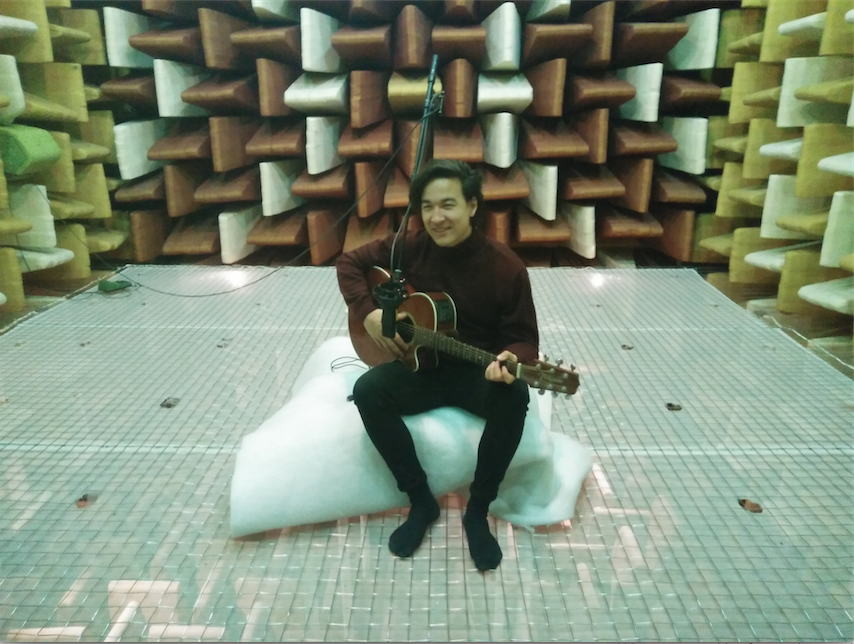
\includegraphics[scale=0.22]{figures/recording/setup1.png}
	\caption{Set up inside anechoic room.}
    \label{fig:setup1}    
    \end{subfigure}
    \begin{subfigure}{0.49\textwidth}
    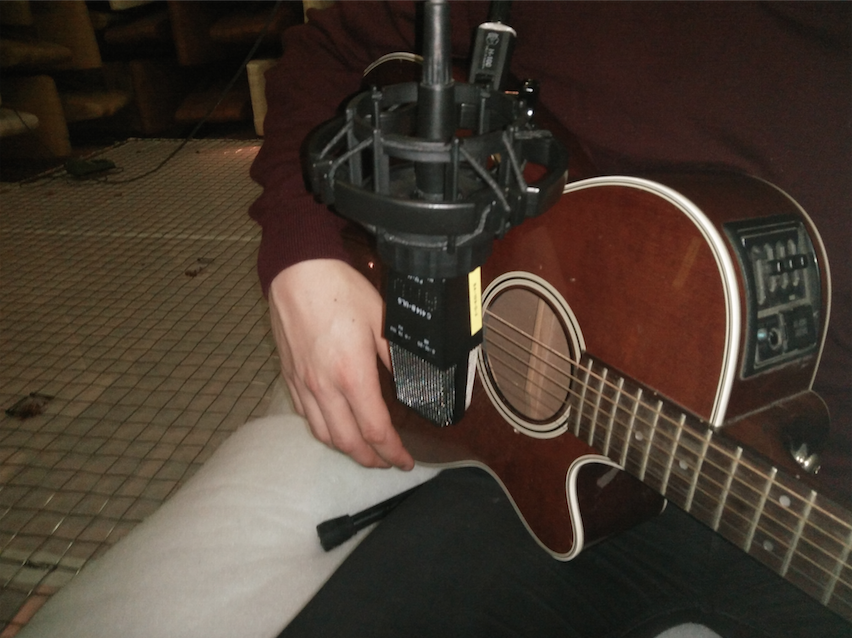
\includegraphics[scale=0.22]{figures/recording/setup2.png}
    \caption{Set up inside anechoic room.}
    \label{fig:setup2}
    \end{subfigure}
\end{figure} 

\textbf{Recording procedure}\\
Through a communications system the guitarist is told what and when to play by the person in the control room, who controls the recordings. At the start of each recording the guitarist says out loud what he is about to play such that there can be no doubt what has been recorded.
The procedure for recording the noise follows the same procedure.
\\ \\
When recording the outdoor ambient noise the microphone stand is placed in an open window inside the control room. One long recording is taken, which include bird song, car noise, and especially noise from a ventilator. A second recording is made with the same premises with a conversation in the background.

\section{Sources of errors}
The following are possible sources of errors made in the recordings.

\begin{itemize}
\item[-] Internal noise from microphone. 
\item[-] Reflections of the signal caused by the floor and the guitarist.
\item[-] Not playing exactly the desired tone.
\item[-] The sensibility/gain adjustments to be made on the ADC was adjusted for the recorded sound to not peak within the frequency band provided by Audacity. If a peak is reached it will cause an error.       
\end{itemize}

\section{Evaluation}
Usable audio files with minimal amount of noise was obtained from the recordings. The noise was minimised by using the anechoic room and furthermore by minimising the amount of equipment and people in the room.
A frequency analysis of the recorded signals is described in chapter~\ref{ch9}.

\clearpage